% Project presentation. Scientific numbers come from explicitly identified snapshots.
% Rebuild: make ncs. Previous progress deck retained in archive/.
\documentclass[aspectratio=169,13pt]{beamer}
\usepackage[T1]{fontenc}
\usepackage[utf8]{inputenc}
\usepackage{lmodern}
\usepackage{amsmath,amssymb,booktabs,graphicx,tikz,array}
\usetikzlibrary{arrows.meta,positioning,calc}
\graphicspath{{figures/}}
\definecolor{teal}{HTML}{087F8C}
\definecolor{ink}{HTML}{173640}
\definecolor{muted}{HTML}{617780}
\definecolor{pale}{HTML}{EDF5F6}
\definecolor{amber}{HTML}{B77818}
\definecolor{sand}{HTML}{FAF3E6}
\setbeamercolor{normal text}{fg=ink,bg=white}
\setbeamercolor{structure}{fg=teal}
\setbeamercolor{frametitle}{fg=ink}
\setbeamercolor{block title}{fg=teal,bg=white}
\setbeamercolor{block body}{fg=ink,bg=white}
\setbeamercolor{alerted text}{fg=amber}
\setbeamerfont{frametitle}{size=\Large,series=\bfseries}
\setbeamerfont{block title}{series=\bfseries}
\setbeamertemplate{navigation symbols}{}
\setbeamertemplate{itemize item}{\color{teal}\small$\bullet$}
\setbeamertemplate{frametitle}{\vspace{.24cm}\insertframetitle\par\vspace{.10cm}\textcolor{teal}{\rule{\linewidth}{.6pt}}}
\setbeamertemplate{footline}{\hspace{.5cm}\color{muted}\scriptsize MetaG\hfill Molecular structure to metabolic thermodynamics\hfill\insertframenumber\hspace{.5cm}\vspace{.18cm}}
\setbeamersize{text margin left=.7cm,text margin right=.7cm}
\newcommand{\dg}{\Delta_r G^{\prime\circ}}
\newcommand{\gap}{\par\vspace{.22cm}}
\newcommand{\takeaway}[1]{\par\vspace{.2cm}\begin{beamercolorbox}[wd=\linewidth,sep=.14cm,rounded=true]{block title}\color{teal}\normalsize\bfseries #1\end{beamercolorbox}}
\newcommand{\slidenote}[1]{\vfill{\footnotesize\color{muted}#1\par}}
\tikzset{card/.style={draw=teal!30,fill=pale,rounded corners=4pt,align=center,inner sep=9pt},arr/.style={-{Latex[length=2.5mm]},thick,teal}}
\title{MetaG}
\subtitle{From molecular structure to metabolic reaction Gibbs energy}
\author{Ray Zhu}
\date{October 2026}
% Generated from presentation_results.json and its local evidence.
\newcommand{\AccuracyNote}{Frozen release 2026-10-01c; archived openTECR labels. Development score; reference conditions are not fully resolved.}
\newcommand{\AccuracySnapshot}{Release 2026-10-01c}
\newcommand{\AccuracySource}{\path{artifacts/results/metag_opentecr_calibrated}}
\newcommand{\ComparisonNote}{302 shared predictions; pretrained baselines and archived labels. 148 match dGbyG training reactions. MetaG replay withholds six phosphorus cases.}
\newcommand{\ComparisonSnapshot}{Audited FD replay}
\newcommand{\ComparisonSource}{\path{artifacts/benchmark/comparison/full_panel_metrics.tsv}}
\newcommand{\MatchedNote}{Structure, direction, and reaction scale matched. dGbyG is out-of-fold; MetaG is a development estimate bridged to I=0.25 M.}
\newcommand{\MatchedSnapshot}{Paper targets}
\newcommand{\MatchedSource}{\path{artifacts/benchmark/paper_reproduction/metag_vs_dgbyg_pairs.tsv}}
\newcommand{\ApplicabilityNote}{Frozen release; 50 reactions from each of six EC classes, absent from TECRDB. No experimental labels: this measures applicability, not accuracy.}
\newcommand{\ApplicabilitySnapshot}{Frozen ModelSEED panel}
\newcommand{\ApplicabilitySource}{\path{artifacts/results/generality_report.json}}
\newcommand{\ComponentNote}{Indolepyruvate anions; same five conformers/state and gas thermal terms. ALPB and SMD are continuum models of water. Diagnostic, not full aqueous Gibbs energy. *Solvation term from DFT.}
\newcommand{\ComponentSource}{\path{analysis/ncs_numerical_validation/evidence_20261008_final/audit.json}}
\newcommand{\AccuracyFigure}{presentation_accuracy.png}
\newcommand{\ComparisonFigure}{presentation_comparison.png}
\newcommand{\MatchedFigure}{presentation_matched.png}
\newcommand{\DomainFigure}{presentation_domain.png}
\newcommand{\StereoFigure}{stereo_check.png}
\newcommand{\ComponentFigure}{presentation_state_gap.png}
\newcommand{\CoreFigure}{coa_core_example.png}
\newcommand{\ReferenceFigure}{reference_coverage.png}
\newcommand{\LearnedScatterFigure}{presentation_learned_scatter.png}
\newcommand{\GroupScatterFigure}{presentation_group_scatter.png}
\newcommand{\ImplementationTests}{600}
\newcommand{\ProtectedArtifacts}{20}
\newcommand{\NetworkCycles}{49}
\newcommand{\NetworkViolations}{11}
\newcommand{\SourceKetoCoverage}{74.48}
\newcommand{\TargetKetoCoverage}{6.50}
\newcommand{\AccuracyN}{364}
\newcommand{\AccuracyScored}{364}
\newcommand{\AccuracyMAE}{9.54}
\newcommand{\AccuracyMedian}{7.15}
\newcommand{\AccuracyRMSE}{13.32}
\newcommand{\SharedN}{302}
\newcommand{\SharedMAE}{8.97}
\newcommand{\StrictMAE}{4.20}
\newcommand{\SharedTrainingOverlap}{148}
\newcommand{\MatchedN}{164}
\newcommand{\MatchedMetaGMAE}{8.66}
\newcommand{\MatchedBaselineMAE}{4.84}
\newcommand{\ElectronicChange}{0.41}
\newcommand{\SolventChange}{23.09}
\newcommand{\LiveReactions}{43{,}669}
\newcommand{\MissingEnergies}{10{,}863}
\newcommand{\UsableMissing}{4{,}307}
\newcommand{\ApplicationN}{300}
\newcommand{\ApplicationScored}{297}
\newcommand{\ApplicationFailed}{3}

\begin{document}

% 1 -------------------------------------------------------------------------
\begin{frame}[plain]
\vspace{.35cm}
{\color{teal}\large Metabolic reaction thermodynamics}\par\vspace{.4cm}
{\Huge\bfseries MetaG}\par\vspace{.25cm}
{\LARGE From molecular structure to\\metabolic reaction Gibbs energy}\par\vspace{.6cm}
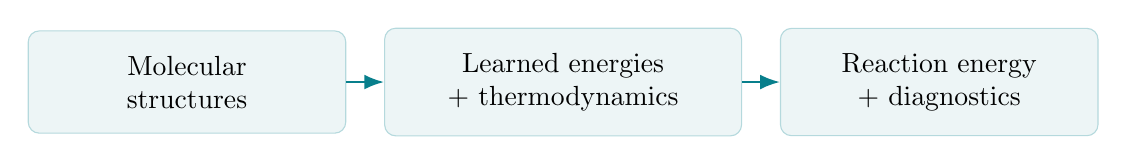
\begin{tikzpicture}[node distance=.48cm]
\node[card,text width=3.4cm,minimum height=1.1cm](a){Molecular\\structures};
\node[card,text width=3.9cm,minimum height=1.1cm,right=of a](b){Learned energies\\+ thermodynamics};
\node[card,text width=3.4cm,minimum height=1.1cm,right=of b](c){Reaction energy\\+ diagnostics};
\draw[arr](a)--(b);\draw[arr](b)--(c);
\end{tikzpicture}
\vfill{\large Ray Zhu\hfill\color{muted}October 2026}
\end{frame}

% 2 -------------------------------------------------------------------------
\begin{frame}{Why thermodynamics matters for metabolism}
\centering
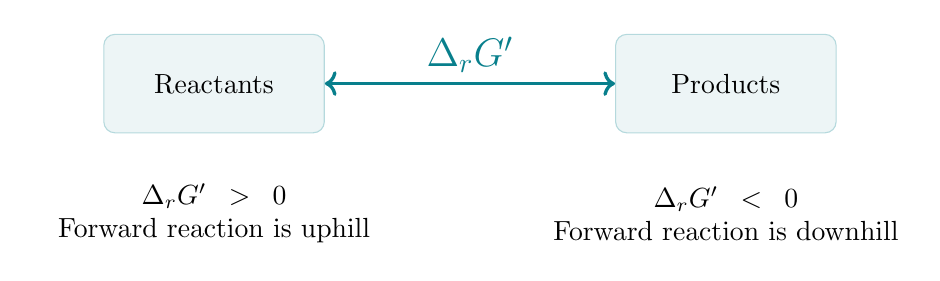
\begin{tikzpicture}
\node[card,minimum width=2.8cm,minimum height=1.25cm](a) at (0,0){Reactants};
\node[card,minimum width=2.8cm,minimum height=1.25cm](b) at (6.5,0){Products};
\draw[<->,teal,very thick](a)--node[above,font=\Large]{$\Delta_r G^\prime$}(b);
\node[align=center,text width=4.5cm] at (0,-1.65){$\Delta_r G^\prime>0$\\Forward reaction is uphill};
\node[align=center,text width=4.5cm] at (6.5,-1.65){$\Delta_r G^\prime<0$\\Forward reaction is downhill};
\end{tikzpicture}
\gap
\begin{columns}[T]
\column{.31\textwidth}\centering\textbf{Reaction direction}\\\small Which way can it run?
\column{.31\textwidth}\centering\textbf{Pathway feasibility}\\\small Where is the bottleneck?
\column{.31\textwidth}\centering\textbf{Metabolic design}\\\small Which route is favorable?
\end{columns}
\slidenote{Concentrations and coupling also affect feasibility; a favorable energy does not imply a fast reaction.}
\end{frame}

% 3 -------------------------------------------------------------------------
\begin{frame}{The thermodynamic map is incomplete}
\centering
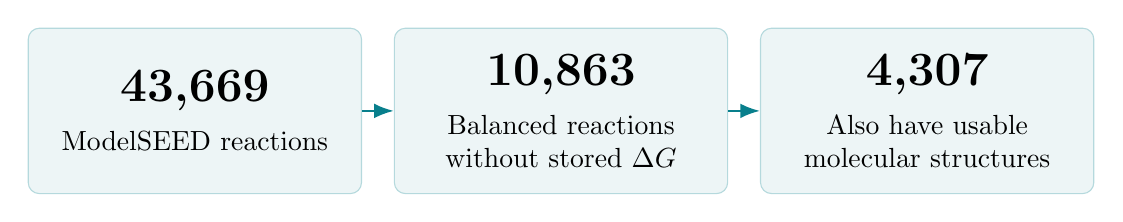
\begin{tikzpicture}
\node[card,text width=3.6cm,minimum height=2.1cm](a) at (0,0){{\LARGE\bfseries \LiveReactions{}}\\[.2cm]ModelSEED reactions};
\node[card,text width=3.6cm,minimum height=2.1cm](b) at (4.65,0){{\LARGE\bfseries \MissingEnergies{}}\\[.2cm]Balanced reactions\\without stored $\Delta G$};
\node[card,text width=3.6cm,minimum height=2.1cm](c) at (9.3,0){{\LARGE\bfseries \UsableMissing{}}\\[.2cm]Also have usable\\molecular structures};
\draw[arr](a)--(b);\draw[arr](b)--(c);
\end{tikzpicture}
\gap\gap
\takeaway{Molecular structures provide another route to reaction energies.}
\slidenote{Local ModelSEED snapshot; live, non-transport reactions. Structural eligibility measures input availability, not accuracy.}
\end{frame}

% 4 -------------------------------------------------------------------------
\begin{frame}{Three routes from chemistry to reaction energy}
\centering
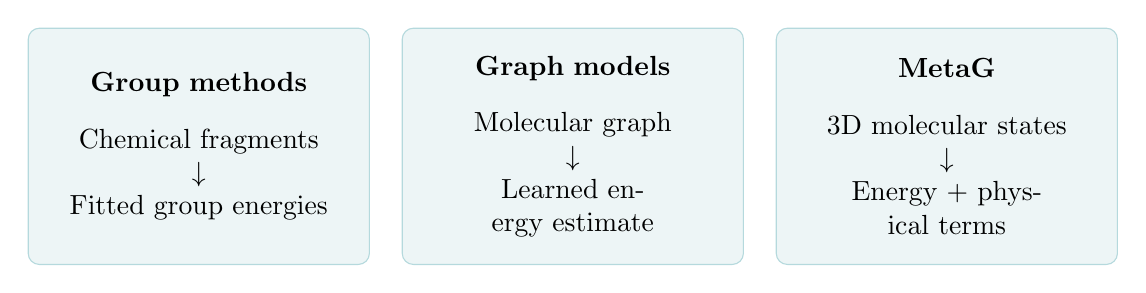
\begin{tikzpicture}
\node[card,text width=3.7cm,minimum height=3cm](a) at (0,0){\textbf{Group methods}\\[.3cm]Chemical fragments\\$\downarrow$\\Fitted group energies};
\node[card,text width=3.7cm,minimum height=3cm](b) at (4.75,0){\textbf{Graph models}\\[.3cm]Molecular graph\\$\downarrow$\\Learned energy estimate};
\node[card,text width=3.7cm,minimum height=3cm](c) at (9.5,0){\textbf{MetaG}\\[.3cm]3D molecular states\\$\downarrow$\\Energy + physical terms};
\end{tikzpicture}
\gap
\takeaway{MetaG makes geometry, chemical states, and energy contributions explicit.}
\slidenote{Examples: eQuilibrator / dGPredictor; dGbyG. UMA supplies MetaG's learned electronic energies and forces.}
\end{frame}

% 5 -------------------------------------------------------------------------
\begin{frame}{A molecular energy is only the starting point}
\centering
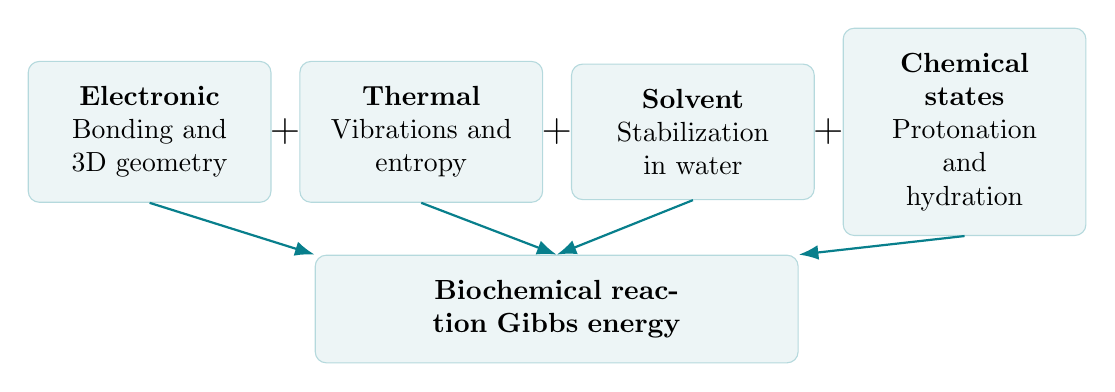
\begin{tikzpicture}
\node[card,text width=2.45cm,minimum height=1.5cm](a) at (0,0){\textbf{Electronic}\\Bonding and\\3D geometry};
\node[card,text width=2.45cm,minimum height=1.5cm](b) at (3.45,0){\textbf{Thermal}\\Vibrations and\\entropy};
\node[card,text width=2.45cm,minimum height=1.5cm](c) at (6.9,0){\textbf{Solvent}\\Stabilization\\in water};
\node[card,text width=2.45cm,minimum height=1.5cm](d) at (10.35,0){\textbf{Chemical states}\\Protonation and\\hydration};
\node[font=\Large] at (1.72,0){+};\node[font=\Large] at (5.17,0){+};\node[font=\Large] at (8.62,0){+};
\node[card,text width=5.5cm,minimum height=.85cm](e) at (5.17,-2.25){\textbf{Biochemical reaction Gibbs energy}};
\draw[arr](a.south)--(e.north west);\draw[arr](b.south)--(e.north);\draw[arr](c.south)--(e.north);\draw[arr](d.south)--(e.north east);
\end{tikzpicture}
\takeaway{The pipeline connects microscopic chemistry to a biochemical quantity.}
\slidenote{UMA is a machine-learned interatomic potential: it predicts energies and forces from 3D structures.}
\end{frame}

% 6 -------------------------------------------------------------------------
\begin{frame}{What quantity does MetaG predict?}
\centering
{\LARGE $\displaystyle\Delta_rG^\prime=\underbrace{\dg}_{\text{MetaG output}}+\underbrace{RT\ln Q^\prime}_{\text{concentration effect}}$}\par\vspace{.45cm}
\begin{columns}[T]
\column{.48\textwidth}
\begin{block}{Standard biochemical conditions}
\small 298.15 K \quad $\vert$ \quad pH 7\\[.2cm]
$I=0$ \quad $\vert$ \quad no Mg binding
\end{block}
\column{.48\textwidth}
\begin{block}{Reaction as written}
\small 1 M solutes; pure liquid water\\[.2cm]
Energy reported in kJ/mol
\end{block}
\end{columns}
\gap
\takeaway{Use the standard energy with concentrations to assess a pathway.}
\slidenote{These conditions are fixed in the pipeline. $Q^\prime$ is the biochemical reaction quotient.}
\end{frame}

% 7 -------------------------------------------------------------------------
\begin{frame}{The pipeline: structures in, reaction energy out}
\centering
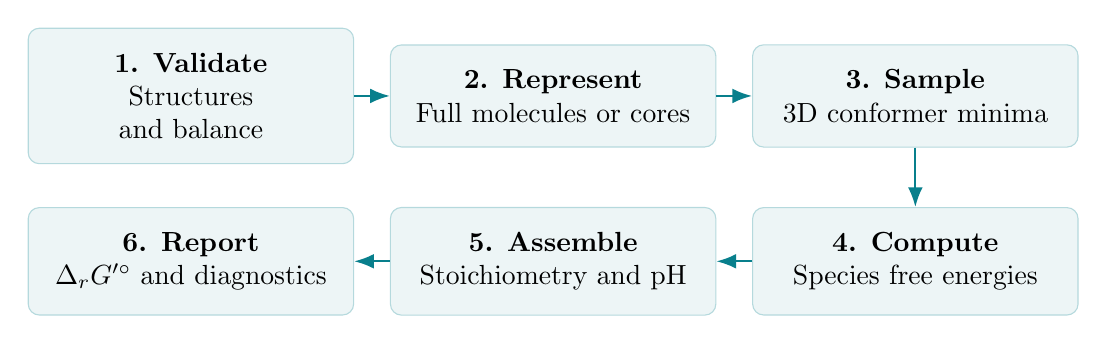
\begin{tikzpicture}[x=1cm,y=1cm]
\node[card,text width=3.5cm,minimum height=1.2cm](a) at (0,0){\textbf{1. Validate}\\Structures and balance};
\node[card,text width=3.5cm,minimum height=1.2cm](b) at (4.6,0){\textbf{2. Represent}\\Full molecules or cores};
\node[card,text width=3.5cm,minimum height=1.2cm](c) at (9.2,0){\textbf{3. Sample}\\3D conformer minima};
\node[card,text width=3.5cm,minimum height=1.2cm](d) at (9.2,-2.1){\textbf{4. Compute}\\Species free energies};
\node[card,text width=3.5cm,minimum height=1.2cm](e) at (4.6,-2.1){\textbf{5. Assemble}\\Stoichiometry and pH};
\node[card,text width=3.5cm,minimum height=1.2cm](f) at (0,-2.1){\textbf{6. Report}\\$\dg$ and diagnostics};
\draw[arr](a)--(b);\draw[arr](b)--(c);\draw[arr](c)--(d);\draw[arr](d)--(e);\draw[arr](e)--(f);
\end{tikzpicture}
\gap\takeaway{Each prediction retains the molecular representation and energy terms.}
\end{frame}

% 8 -------------------------------------------------------------------------
\begin{frame}{One molecule can occupy several 3D conformations}
\centering
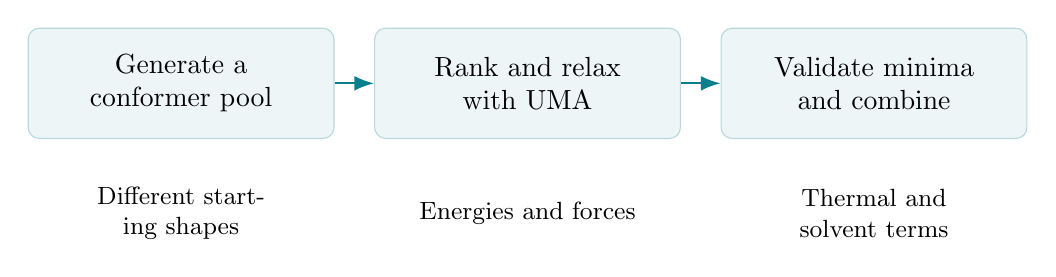
\begin{tikzpicture}
\node[card,text width=3.25cm,minimum height=1.4cm](a) at (0,0){Generate a\\conformer pool};
\node[card,text width=3.25cm,minimum height=1.4cm](b) at (4.4,0){Rank and relax\\with UMA};
\node[card,text width=3.25cm,minimum height=1.4cm](c) at (8.8,0){Validate minima\\and combine};
\draw[arr](a)--(b);\draw[arr](b)--(c);
\node[text width=3.4cm,align=center,font=\small] at (0,-1.65){Different starting shapes};
\node[text width=3.4cm,align=center,font=\small] at (4.4,-1.65){Energies and forces};
\node[text width=3.4cm,align=center,font=\small] at (8.8,-1.65){Thermal and solvent terms};
\end{tikzpicture}
\gap
\takeaway{An ensemble includes both low-energy structures and their populations.}
\slidenote{Sampling expands until the calculated ensemble stabilizes. A plateau does not bound undiscovered conformers.}
\end{frame}

% 9 -------------------------------------------------------------------------
\begin{frame}{From conformers to species, then to reactions}
\begin{columns}[c]
\column{.48\textwidth}
\centering\textbf{Within a species}\gap
$g_k=E_k^{\rm UMA}+G_k^{\rm thermal}+\Delta G_k^{\rm solvent}$\gap
$\displaystyle G_i=-RT\ln\sum_k e^{-g_k/RT}+C^\circ$\gap
\small Low-energy conformers carry more weight.
\column{.48\textwidth}
\centering\textbf{Across a reaction}\gap
$\displaystyle\dg=\sum_i\nu_iG_i^{\rm eff}+C_{\rm proton/pH}$\gap
\small Products add; reactants subtract.\\[.15cm]
$G_i^{\rm eff}$ also includes enabled hydrate states.
\end{columns}
\gap\takeaway{Every reaction energy can be traced back to its molecular contributions.}
\slidenote{$C^\circ$: standard-state correction. The appendix gives the proton, water, and pKa conventions.}
\end{frame}

% 10 ------------------------------------------------------------------------
\begin{frame}{Large cofactors: retain the chemistry that changes}
\centering\includegraphics[width=.97\linewidth,height=4.25cm,keepaspectratio]{\CoreFigure}
\takeaway{The structural core preserves the reactive thioester and its local scaffold.}
\slidenote{CoA example from the router. Balance and removed-fragment identity are checked; cores remain approximations.}
\end{frame}

% 11 ------------------------------------------------------------------------
\begin{frame}{The aqueous species is a mixture of chemical states}
\centering
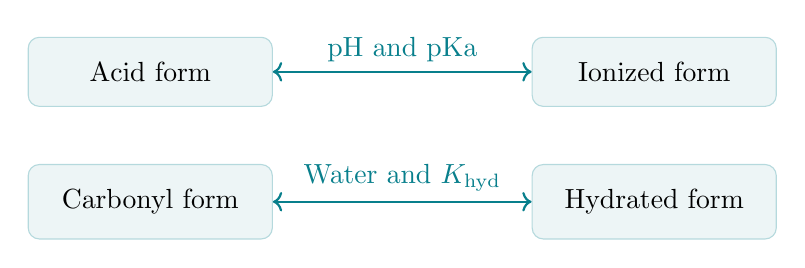
\begin{tikzpicture}
\node[card,minimum width=3.1cm,minimum height=.85cm](a) at (0,0){Acid form};
\node[card,minimum width=3.1cm,minimum height=.85cm](b) at (6.4,0){Ionized form};
\node[card,minimum width=3.1cm,minimum height=.85cm](c) at (0,-1.65){Carbonyl form};
\node[card,minimum width=3.1cm,minimum height=.85cm](d) at (6.4,-1.65){Hydrated form};
\draw[<->,teal,thick](a)--node[above]{pH and pKa}(b);
\draw[<->,teal,thick](c)--node[above]{Water and $K_{\rm hyd}$}(d);
\end{tikzpicture}
\gap
\takeaway{State populations shift the effective free energy of a metabolite.}
\slidenote{Production uses independent pKa sites and enabled carbonyl hydration. The two equilibria are schematic; coupled-state routing is not assumed.}
\end{frame}

\begin{frame}{Current scoring and the new validation tools}
\begin{columns}[T]
\column{.48\textwidth}
\begin{block}{Active reaction scorer}
\small UMA + gas thermal terms + ALPB.\gap
Tabulated pKa patterns; largely independent sites.\gap
Unsupported isotope inputs are withheld; the legacy SMD reaction correction is blocked.
\end{block}
\column{.48\textwidth}
\begin{block}{Implemented research tools}
\small Coupled-state registry: references, conditions, and thermodynamic cycles.\gap
Aqueous-ensemble admission and network/covariance audits.\gap
These tools do not replace the default energy or pKa model.
\end{block}
\end{columns}
\takeaway{The package now checks more assumptions; its default pKa physics is unchanged.}
\slidenote{Integration snapshot: 8 October 2026. Registry transitions require justified state-specific data; the registry does not predict missing pKa values.}
\end{frame}

% 12 ------------------------------------------------------------------------
\begin{frame}{Benchmark design separates three questions}
\centering
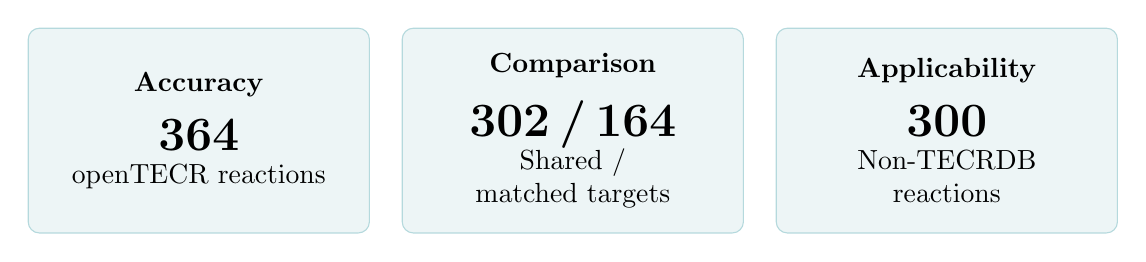
\begin{tikzpicture}
\node[card,text width=3.7cm,minimum height=2.6cm](a) at (0,0){\textbf{Accuracy}\\[.25cm]{\LARGE\bfseries 364}\\openTECR reactions};
\node[card,text width=3.7cm,minimum height=2.6cm](b) at (4.75,0){\textbf{Comparison}\\[.25cm]{\LARGE\bfseries 302 / 164}\\Shared / matched targets};
\node[card,text width=3.7cm,minimum height=2.6cm](c) at (9.5,0){\textbf{Applicability}\\[.25cm]{\LARGE\bfseries 300}\\Non-TECRDB reactions};
\end{tikzpicture}
\gap
\takeaway{Prediction accuracy, relative performance, and coverage are different tests.}
\slidenote{Accuracy uses frozen development predictions and archived references; the 300-reaction panel has no experimental energy labels.}
\end{frame}

% 13 ------------------------------------------------------------------------
\begin{frame}{openTECR: a \AccuracyMAE{} kJ/mol mean absolute error}
\begin{columns}[c]
\column{.56\textwidth}\centering\includegraphics[width=\linewidth,height=4.9cm,keepaspectratio]{\AccuracyFigure}
\column{.40\textwidth}
{\LARGE\bfseries\color{teal}9.54}\quad kJ/mol\\\small Mean absolute error\gap
{\Large\bfseries 7.15}\quad kJ/mol\\\small Median absolute error\gap
{\Large\bfseries \AccuracyScored{} / \AccuracyN{}}\\\small Reactions scored
\end{columns}
\slidenote{\AccuracyNote{}}
\end{frame}

% 14 ------------------------------------------------------------------------
\begin{frame}{Shared-reaction comparison: accuracy and coverage}
\centering\includegraphics[width=\linewidth,height=4.2cm,keepaspectratio]{\ComparisonFigure}
\takeaway{Fitted baselines have lower error on this benchmark.}
\slidenote{\ComparisonNote{}}
\end{frame}

\begin{frame}{Shared targets: MetaG, dGbyG and dGPredictor}
\centering\includegraphics[width=\linewidth,height=4.75cm,keepaspectratio]{\LearnedScatterFigure}
\takeaway{The same \SharedN{} reactions and axis limits are used for every method.}
\slidenote{Archived labels; MetaG historical FD replay and pretrained baselines. dGbyG uses an eQuilibrator bridge; \SharedTrainingOverlap{} / \SharedN{} targets match its training reactions. This comparison is not held out.}
\end{frame}

\begin{frame}{Shared targets: MetaG and eQuilibrator}
\centering\includegraphics[width=\linewidth,height=4.75cm,keepaspectratio]{\GroupScatterFigure}
\takeaway{Component contribution closely reproduces these archived references.}
\slidenote{CC: component contribution; GC-only: group contribution. Diagonal: agreement. Archived labels; unresolved conditions and training overlap. This comparison is not held out.}
\end{frame}

% 15 ------------------------------------------------------------------------
\begin{frame}{Matched targets: held-out dGbyG is more accurate}
\centering\includegraphics[width=.96\linewidth,height=4.15cm,keepaspectratio]{\MatchedFigure}
\takeaway{MAE: MetaG \MatchedMetaGMAE{} vs dGbyG \MatchedBaselineMAE{} kJ/mol on \MatchedN{} targets.}
\slidenote{Structure, direction, and reaction scale matched. dGbyG is out-of-fold; MetaG is a development estimate bridged to $I=0.25$ M.}
\end{frame}

% Significance ---------------------------------------------------------------
\begin{frame}{The benchmark covers little of the unfamiliar chemistry}
\centering\includegraphics[width=.94\linewidth,height=3.65cm,keepaspectratio]{\DomainFigure}
\takeaway{The benchmark contains little of ModelSEED's least familiar chemistry.}
\slidenote{Fraction containing an unseen compound with nearest-training Tanimoto $<0.5$. Denominators: all balanced ModelSEED reactions vs openTECR. Novelty is not an accuracy measurement.}
\end{frame}

\begin{frame}{Why MetaG matters alongside a strong dGbyG}
\centering
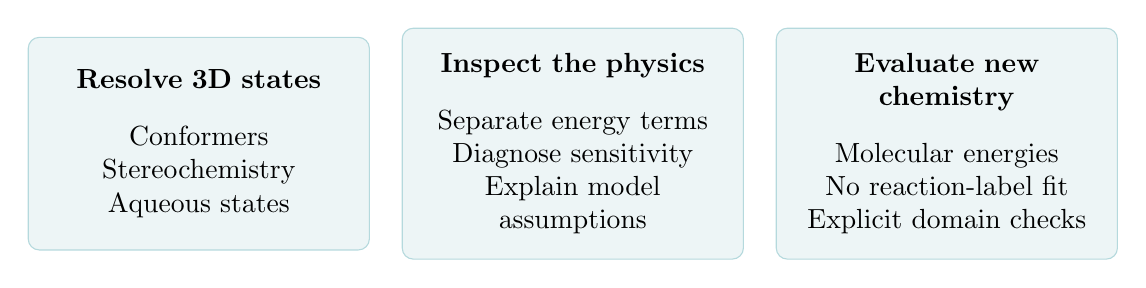
\begin{tikzpicture}
\node[card,text width=3.7cm,minimum height=2.7cm](a) at (0,0){\textbf{Resolve 3D states}\\[.3cm]Conformers\\Stereochemistry\\Aqueous states};
\node[card,text width=3.7cm,minimum height=2.7cm](b) at (4.75,0){\textbf{Inspect the physics}\\[.3cm]Separate energy terms\\Diagnose sensitivity\\Explain model assumptions};
\node[card,text width=3.7cm,minimum height=2.7cm](c) at (9.5,0){\textbf{Evaluate new chemistry}\\[.3cm]Molecular energies\\No reaction-label fit\\Explicit domain checks};
\end{tikzpicture}
\gap\takeaway{MetaG adds a physical route to estimation and diagnosis.}
\slidenote{Complementary capabilities motivate the workflow. Higher accuracy on unfamiliar reactions is not established.}
\end{frame}

% 16 ------------------------------------------------------------------------
\begin{frame}{Geometry resolves differences between stereoisomers}
\centering\includegraphics[width=\linewidth,height=4.1cm,keepaspectratio]{\StereoFigure}
\takeaway{UMA reproduces the opposite E/Z orderings of these two gas-phase pairs.}
\slidenote{2-butene and 1,2-difluoroethylene. MMFF94 gives the wrong sign for the latter. This component test measures gas-phase energetics.}
\end{frame}

% 17 ------------------------------------------------------------------------
\begin{frame}{Energy decomposition identifies solvent sensitivity}
\centering\includegraphics[width=.91\linewidth,height=3.65cm,keepaspectratio]{\ComponentFigure}
\begin{columns}[T]
\column{.48\textwidth}\centering\textbf{Electronic model change}\\\color{teal}{\large \ElectronicChange{} kJ/mol}\quad\small with ALPB
\column{.48\textwidth}\centering\textbf{Solvent model change}\\\color{teal}{\large \SolventChange{} kJ/mol}\quad\small with DFT
\end{columns}
\slidenote{\ComponentNote{}}
\end{frame}

\begin{frame}{Solvent changes which conformers matter}
\begin{columns}[T]
\column{.48\textwidth}
\begin{block}{Same five saved keto conformers}
\small The two source-selected conformers carry:\gap
{\Large\color{teal}\SourceKetoCoverage{}\%}\quad under UMA/ALPB\gap
{\Large\color{amber}\TargetKetoCoverage{}\%}\quad under DFT/SMD\gap
Source selection misses most target-model weight in this fixed set.
\end{block}
\column{.48\textwidth}
\begin{block}{Destination-ensemble audit}
\small Two of three local SMD relaxations meet the force criterion; one reaches the step cap.\gap
Destination Hessians and thermal terms are absent; starts remain missing.\gap
No aqueous Gibbs ensemble or validated interval is admitted.
\end{block}
\end{columns}
\takeaway{Force convergence alone does not validate an aqueous free energy.}
\slidenote{Indolepyruvate keto/Z-enol anions. Fixed-set weights retain gas thermal terms; they are diagnostics, not experimental populations or complete aqueous coverage.}
\end{frame}

% 18 ------------------------------------------------------------------------
\begin{frame}{ModelSEED: \ApplicationScored{} estimates from \ApplicationN{} new reactions}
\centering
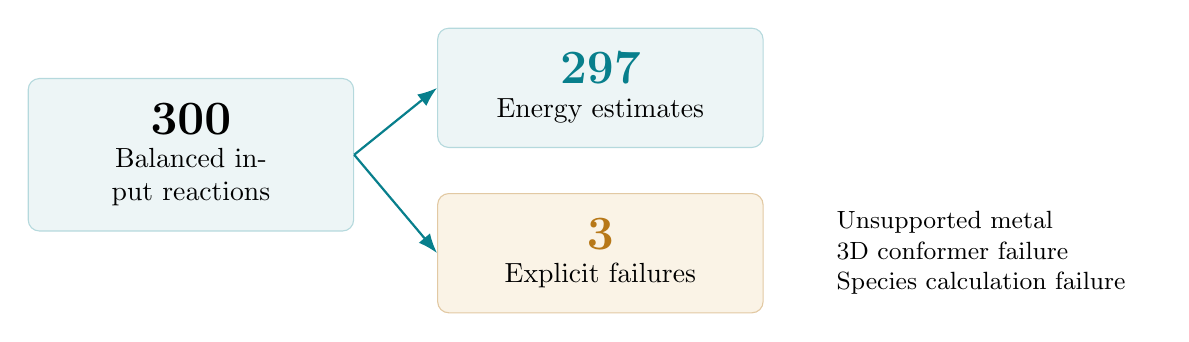
\begin{tikzpicture}
\node[card,text width=3.5cm,minimum height=1.4cm](a) at (0,0){{\LARGE\bfseries 300}\\Balanced input reactions};
\node[card,text width=3.5cm,minimum height=1.4cm](b) at (5.2,.85){{\LARGE\bfseries\color{teal}297}\\Energy estimates};
\node[draw=amber!40,fill=sand,rounded corners,text width=3.5cm,align=center,inner sep=9pt,minimum height=1.4cm](c) at (5.2,-1.25){{\LARGE\bfseries\color{amber}3}\\Explicit failures};
\draw[arr](a.east)--(b.west);\draw[arr](a.east)--(c.west);
\node[text width=4cm,align=left,font=\small] at (10.2,-1.25){Unsupported metal\\3D conformer failure\\Species calculation failure};
\end{tikzpicture}
\gap\takeaway{The workflow processes broader chemistry and retains failed cases.}
\slidenote{\ApplicabilityNote{}}
\end{frame}

% 19 ------------------------------------------------------------------------
\begin{frame}{What determines the reliability of an estimate?}
\centering
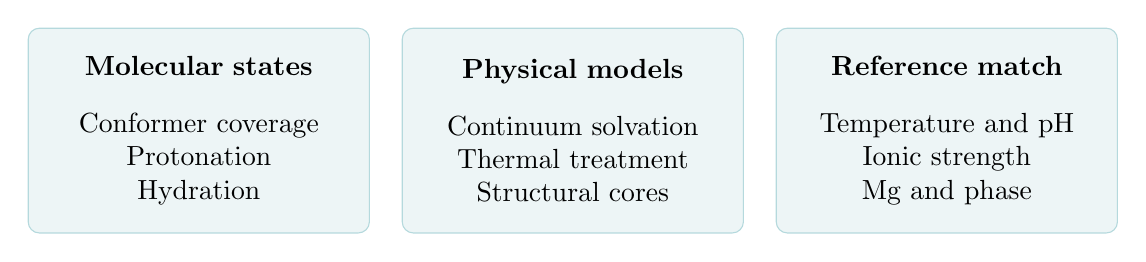
\begin{tikzpicture}
\node[card,text width=3.7cm,minimum height=2.6cm](a) at (0,0){\textbf{Molecular states}\\[.3cm]Conformer coverage\\Protonation\\Hydration};
\node[card,text width=3.7cm,minimum height=2.6cm](b) at (4.75,0){\textbf{Physical models}\\[.3cm]Continuum solvation\\Thermal treatment\\Structural cores};
\node[card,text width=3.7cm,minimum height=2.6cm](c) at (9.5,0){\textbf{Reference match}\\[.3cm]Temperature and pH\\Ionic strength\\Mg and phase};
\end{tikzpicture}
\gap\takeaway{Diagnostics make these assumptions visible in each result.}
\slidenote{OpenTECR development scores do not establish independent chemical transfer; unsupported phosphorus assignments are withheld.}
\end{frame}

\begin{frame}{Network audits expose unresolved consistency}
\begin{columns}[T]
\column{.48\textwidth}
\begin{block}{Frozen historical release}
\small \NetworkCycles{} independent reaction cycles audited.\gap
{\Large\color{amber}\NetworkViolations{}}\quad exceed stated rounding bounds.\gap
Context-dependent molecular representations are retained for inspection.
\end{block}
\column{.48\textwidth}
\begin{block}{New audit capabilities}
\small Partition by chemical state, conditions, and computational settings.\gap
Preserve failed cases and uncertainty provenance.\gap
Propagate supplied shared-state covariance; none is inferred from scalar intervals.
\end{block}
\end{columns}
\takeaway{The audit identifies inconsistency; the reaction energies remain unrepaired.}
\slidenote{Historical diagnostic, not a new accuracy evaluation. No independently validated covariance or external interval-coverage result is available.}
\end{frame}

% 20 ------------------------------------------------------------------------
\begin{frame}{MetaG: molecular physics for metabolic thermodynamics}
\begin{columns}[T]
\column{.49\textwidth}
\begin{block}{The method}
\begin{itemize}
\item Geometry-resolved species energies
\item Physical biochemical corrections
\item Traceable estimates and failures
\end{itemize}
\end{block}
\column{.47\textwidth}
\begin{block}{The evidence}
\begin{itemize}
\item \AccuracyMAE{} kJ/mol development MAE
\item \ApplicationScored{} / \ApplicationN{} applicability estimates
\item Component tests and network audits
\item \ImplementationTests{} passing software tests
\end{itemize}
\end{block}
\end{columns}
\gap\takeaway{A complementary physical estimator with inspectable chemical assumptions.}
\slidenote{MAE and applicability are frozen historical results. Current safeguards and research tools have not established improved overall accuracy or independent transfer.}
\end{frame}

\appendix
% A1 ------------------------------------------------------------------------
\begin{frame}{Appendix: which information is learned or empirical?}
\begin{columns}[T]
\column{.31\textwidth}\begin{block}{Electronic model}\small UMA is trained on quantum-chemical data. Inputs include geometry, charge, and spin.\end{block}
\column{.31\textwidth}\begin{block}{Auxiliary properties}\small pKa references, experimental water hydration, and a component calibration to carbonyl hydration constants.\end{block}
\column{.31\textwidth}\begin{block}{Reaction labels}\small openTECR informs evaluation, interval calibration, and method development.\end{block}
\end{columns}
\gap\takeaway{No openTECR reaction-energy offset is fitted in the point estimate.}
\slidenote{Benchmark-informed routing makes the reported MetaG accuracy a development score. Class anchor corrections are disabled.}
\end{frame}

\begin{frame}{Appendix: implementation validation and scientific scope}
\begin{columns}[T]
\column{.48\textwidth}
\begin{block}{Verified implementation}
\small \ImplementationTests{} passing software tests; package wheel built.\gap
\ProtectedArtifacts{} protected benchmark artifacts unchanged.\gap
Optional solvent relaxation rejects failed gradients, incomplete starts, and unconverged results; it remains off by default.
\end{block}
\column{.48\textwidth}
\begin{block}{Boundaries of that evidence}
\small The strict SMD component API has CPU boundary tests; its new wrapper has no fresh GPU numerical validation.\gap
Coupled pKa scoring, complete aqueous thermodynamics, adaptive core corrections, and deployed shared-state covariance remain unresolved.
\end{block}
\end{columns}
\takeaway{Software tests do not establish reaction accuracy.}
\slidenote{Integration and track sources: \path{presentation_results.json}. Validation record dated 8 October 2026.}
\end{frame}

% A2 ------------------------------------------------------------------------
\begin{frame}{Appendix: reference curation and strict comparison}
\begin{columns}[c]
\column{.52\textwidth}\includegraphics[width=\linewidth,height=3.8cm,keepaspectratio]{\ReferenceFigure}
\column{.44\textwidth}
\textbf{Condition checks}\gap
\small Free Mg activity; constant definition; measured temperature; ionic strength.\gap
\textbf{Strict shared subset}\gap
\small Six reactions: MetaG MAE \StrictMAE{} kJ/mol. All six overlap dGbyG training.
\end{columns}
\slidenote{54 reactions retain curated labels; eight have a row at 298.15 K with reported ionic strength. The small shared subset is descriptive.}
\end{frame}

% A3 ------------------------------------------------------------------------
\begin{frame}{Appendix: energy and standard-state conventions}
\small
\[
\dg=\sum_i\nu_iG_i^{\rm eff}+n_{\rm H^+}G_{\rm H^+}+\sum_j s_jm_j\Delta G_j^{\rm pKa}
\]
\begin{align*}
G_i&=-RT\ln\sum_k\exp[-(E_k^{\rm UMA}+G_k^{\rm RRHO}+\Delta G_k^{\rm ALPB})/RT]+RT\ln24.46\\
G_i^{\rm eff}&=-RT\ln\left[e^{-G_i/RT}+\sum_S e^{-(G_S-n_SG_{\rm w})/RT}\right]
\end{align*}
\begin{columns}[T]
\column{.48\textwidth}\small\textbf{Thermal terms}\gap Zero-point energy and ideal-gas RRHO; UMA Hessian; 50 cm$^{-1}$ frequency floor; symmetry and linearity.
\column{.48\textwidth}\small\textbf{Reservoir conventions}\gap 1 atm $\to$ 1 M: +7.93 kJ/mol.\\Pure-water concentration: +9.96 kJ/mol.\\Proton at pH 7: $-1170.8$ kJ/mol.
\end{columns}
\slidenote{Hydrate terms subtract consumed water. $s_j$: reaction side; $m_j$: site multiplicity. Experimental water hydration: $-26.4$ kJ/mol.}
\end{frame}

% A4 ------------------------------------------------------------------------
\begin{frame}{Appendix: benchmark snapshots and comparison regimes}
\small\renewcommand{\arraystretch}{1.8}
\begin{tabular}{@{}>{\raggedright\arraybackslash}p{3.5cm}>{\raggedright\arraybackslash}p{3.5cm}>{\raggedright\arraybackslash}p{6.0cm}@{}}
\toprule
Result & Snapshot / set & Interpretation\\\midrule
Full-panel MAE \AccuracyMAE{} & \AccuracySnapshot{}; \AccuracyN{} & Archived labels; development accuracy\\
Shared-set MAE \SharedMAE{} & \ComparisonSnapshot{}; \SharedN{} & Different coverage; pretrained baselines\\
Matched-set MAE \MatchedMetaGMAE{} & \MatchedN{} paper targets & MetaG development vs dGbyG out-of-fold\\
\ApplicationScored{} / \ApplicationN{} estimates & \ApplicabilitySnapshot{} & Applicability without energy labels\\\bottomrule
\end{tabular}
\gap
\small Later validation changes are not assigned the frozen release's numerical performance.
\slidenote{Condition bridges use eQuilibrator dissociation data. These comparisons do not establish a matched held-out ranking for MetaG.}
\end{frame}

% A5 ------------------------------------------------------------------------
\begin{frame}{Appendix: component checks and their scope}
\begin{columns}[T]
\column{.48\textwidth}\begin{block}{Stereoisomer check}\small Gas-phase 2-butene enthalpy and difluoroethylene electronic-energy differences.\gap The published dGbyG encoding also collides for tested E/Z and diastereomer inputs.\end{block}
\column{.48\textwidth}\begin{block}{Solvent component check}\small Identical saved indolepyruvate geometries; direct $\omega$B97M-V/def2-TZVPD; ALPB vs SMD.\gap CPU/GPU, grid, and overlap changes are below 0.04 kJ/mol in the tested gaps.\end{block}
\end{columns}
\gap\takeaway{Component evidence explains sensitivity; it does not establish aqueous accuracy.}
\slidenote{Gas thermal terms are retained in the solvent comparison. Numerical agreement checks implementation consistency.}
\end{frame}

% A6 ------------------------------------------------------------------------
\begin{frame}{Appendix: evidence and reproducibility}
\small
\textbf{Local evidence (relative to the project directory)}\gap
\begin{tabular}{@{}>{\raggedright\arraybackslash}p{3.6cm}>{\raggedright\arraybackslash}p{9.7cm}@{}}
Accuracy & \AccuracySource\\[.12cm]
Baseline metrics & \ComparisonSource\\[.12cm]
Matched targets & \MatchedSource\\[.12cm]
ModelSEED applicability & \ApplicabilitySource\\[.12cm]
\end{tabular}
\gap\footnotesize
Database scope and component sources are indexed in \path{presentation_results.json}.
\gap\footnotesize
Fan et al., Cell Systems (2025), \href{https://doi.org/10.1016/j.cels.2025.101393}{doi:10.1016/j.cels.2025.101393}.\quad
\href{https://arxiv.org/abs/2505.08762}{OMol25}.\\
Beber et al., eQuilibrator 3.0, \href{https://doi.org/10.1093/nar/gkab1106}{doi:10.1093/nar/gkab1106}.\\
Stereo references: Prosen et al. (1951); Craig et al. (1971), Table II.
\slidenote{Build: make ncs. New presentation figures: make\_presentation\_figures.py. Scientific figures derive from preserved local evidence.}
\end{frame}

\end{document}
